\newpage
\subsection{Aktuator interface - Jens}
Aktuator interfacet er bindeledet imellem PSoC3 og de fysiske aktuatore. Da der ikke er forskel på hvordan aktuator drives i systemet er der i det følgende afsnit kun beskrevet generelt.   

\subsubsection{Design}
Der er flere måder at foretage styringen af aktuatoreren på, dette kunne fx. være via relæ, solid state relæ, effekt transistor, MOSFET eller Darlington array.  

Til at trække stepmorten, magnetventilen, samt de to blæsere faldt designvalget på et Darlington array. 

Dette designvalg blev truffet på baggrund af følgende overvejelser.
\begin{itemize}
	\item Relæet ville ikke være optimal til PWM sammenhæng pga. det store mekaniske slid dette ville medføre på relækontaktorerne, det er heller ikke muligt at køre med en ret høj PWM frekvens pga. spolen i relæet.
	\item Solid state relæ kunne havde været en mulighed, da der ikke er noget mekaniske slid i denne form for relæer. Solid state relæ blev valgt fra pga. prisen og den fysiske byggestørrelse på komponenten.
	\item Effekttransistor har en lille forstærkning hvilket ville kræve en støre strøm end de 4mA PSoC3 er i stand til at levere på dens udgange, derfor blev denne fravalgt. 
	\item MOSFETen kunne have været et oplagt valg, men blev valgt fra da det ønskes at holde antallet af elektriske komponenter på et minimum, hvilket et darlington array muliggøre. 
\end{itemize} 

\subsubsection{Implementering}
Aktuator interfacet er implementeret med to Darlington arrays af typen ULN2001 (figur \ref{fig:ULN2001_princip} viser princippet vha. et diagram). Grunden til at der er anvendt to Darlington arrays er at der avendes to forskellige spændinger i systemet, hhv. 5VDC til stepmotoren og 12VDC til blæser samt magnetventilen. 
Denne type Darlington array indholder 7 undgange der hver er i stand til at trække en strøm på 500mA. Det er muligt at parallel koble disse udgangs strømme. Denne egenskab udnyttes således at det er muligt at trække magnetventilen der trækker strøm på 1A. På hver indgang er der monteret en 2.7k$\Omega$ modstand for at tilpasse indgangsstrømmen til 5VDC CMOS kredse. 
\begin{figure}[H]
\centering
{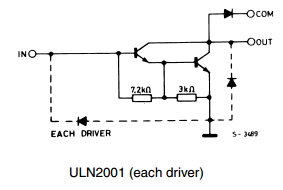
\includegraphics[page=1,scale=0.9,trim=5mm 5mm 5mm 5mm]{./7_projektbeskrivelse/design_og_implementering/hardware/ULN2001_prencip.png}}
\caption[Figur]{$1/7$ af ULN2001}
\label{fig:ULN2001_princip}
\end{figure}